\chapter{Resultados}
\label{cap:resultados}

\section{Classificação de Tipo de Superfície de Pista}

Todos os modelos desenvolvidos neste estudo foram programados em Python 3. Os modelos de Classical Machine Learning utilizaram da biblioteca Scikit-Learn, enquanto que os de Deep Learning utilizaram do framework Keras com backend Tensorflow. Os experimentos foram executados no Google Colab, em uma GPU NVIDIA Tesla P100 com 12 GB e 25 GB RAM. Com exceção do KNN, em todas as outras técnicas os experimentos foram executados 3 vezes para minimizar a aleatoriedade dos parâmetros iniciais, recuperando-se apenas o melhor entre eles. Considerou-se como melhor modelo, aquele que apresentou maior valor de acurácia no dataset de validação. Os resultados obtidos na aplicacão de Classical Machine Learning são detalhados nas Tabelas \ref{table:kmc_results}, \ref{table:svm_results} e \ref{table:knn_results}. O valor exibido corresponde a média de acurácia no dataset de validação dos três experimentos para dado tamanho de janela de dados e configuração de hiper-parâmetros da técnica.

\begin{table}[h!]
\caption{Valores de acurácia de validação para o KMC.} 
\label{table:kmc_results}
\centering
\small
\begin{tabular}{ccccccc}
\cmidrule(l){2-6}
\textbf{} & \multicolumn{5}{c}{\textbf{Janela}} \\ \midrule
\textbf{Clusters} & \textbf{100} & \textbf{150} & \textbf{200} & \textbf{250} & \textbf{300} & \textbf{Média} \\ \midrule
3 & 56.20\% & 58.13\% & 59.10\% & 59.67\% & \textbf{60.42\%} & 58.70\% \\ \bottomrule
\end{tabular}
\end{table}

\begin{table}[h!]
\caption{Valores de acurácia de validação para o SVM.} 
\label{table:svm_results}
\centering
\small
\begin{tabular}{ccccccc}
\cmidrule(l){2-6}
\textbf{} & \multicolumn{5}{c}{\textbf{Janela}} \\ \midrule
\textbf{Kernel} & \textbf{100} & \textbf{150} & \textbf{200} & \textbf{250} & \textbf{300} & \textbf{Média} \\ \midrule
poly 3 & 65.00\% & 66.60\% & 68.05\% & 68.07\% & \textbf{68.71\%} & 67.28\% \\ \midrule
rbf & 71.95\% & 72.28\% & \textbf{72.68\%} & 72.42\% & 72.45\% & 72.36\% \\ \midrule
sigmoid & 52.80\% & 47.08\% & \textbf{57.50\%} & 54.73\% & 56.75\% & 53.77\% \\ \midrule
\textbf{Média} & 63.25\% & 61.99\% & 66.08\% & 65.08\% & 65.97\% & 64.47\% \\ \bottomrule
\end{tabular}
\end{table}

\begin{table}[h!]
\caption{Valores de acurácia de validação para o KNN.} 
\label{table:knn_results}
\centering
\small
\begin{tabular}{ccccccc}
\cmidrule(l){2-6}
\textbf{} & \multicolumn{5}{c}{\textbf{Janela}} \\ \midrule
\textbf{Neighbors} & \textbf{100} & \textbf{150} & \textbf{200} & \textbf{250} & \textbf{300} & \textbf{Média} \\ \midrule
1 & 72.28\% & 72.77\% & \textbf{74.46\%} & 73.45\% & 73.83\% & 73.36\% \\ \midrule
2 & 59.80\% & 61.08\% & \textbf{62.69\%} & 60.87\% & 61.92\% & 61.27\% \\ \midrule
5 & 72.37\% & 72.78\% & \textbf{74.79\%} & 73.80\% & 73.97\% & 73.54\% \\ \midrule
10 & 67.97\% & 68.39\% & \textbf{70.23\%} & 68.81\% & 69.72\% & 69.02\% \\ \midrule
50 & 70.83\% & 71.54\% & \textbf{72.01\%} & 71.30\% & 69.66\% & 71.07\% \\ \midrule
100 & 69.40\% & \textbf{69.75\%} & 69.47\% & 68.77\% & 67.63\% & 69.00\% \\ \midrule
250 & \textbf{66.25\%} & 65.18\% & 63.84\% & 62.61\% & 61.24\% & 63.83\%\\ \midrule
500 & \textbf{62.15\%} & 59.57\% & 57.66\% & 54.65\% & 53.93\% & 57.59\% \\ \midrule
1000 & \textbf{54.93\%} & 51.42\% & 49.12\% & 45.83\% & 44.05\% & 49.07\% \\ \midrule
\textbf{Média} & 66.22\% & 65.83\% & 66.03\% & 64.45\% & 63.99\% & 65.31\% \\ \bottomrule
\end{tabular}
\end{table}

Para a técnica de KMC, o melhor modelo resultante para 3 clusters é o de janela com 300 amostras, alcançando 58.24\% de acurácia de treinamento e 60.42\% de validação. Nesta técnica, quando maior a janela aplicada, maiores os valores de acurácia encontrados. Na técnica de SVM, o kernel sigmoid apresentou os piores valores para todas as janelas de dados, seguido pelo kernel polinomial de grau 3. Sendo assim, o kernel rbf obteve os melhores valores de acurácia para todas as variações de janela, e o modelo com 200 amostras obteve acurácia de 76.15\% para treinamento e 72.68\% para validação. Neste kernel, o tamanho da janela de dados tem pouca influência no resultado final. Por fim, o KNN apresenta melhores resultados com a quantidade de vizinhos entre 1-50, onde o tamanho da janela também não apresenta grande influência no resultado. Já com grandes quantidades de vizinhos, o resultado tende a apresentar uma maior variação conforme a quantidade de amostras. Para a quantidade de vizinhos entre 1-50, a janela com 200 amostras apresenta melhores resultados, situando o melhor modelo com 5 vizinhos, onde obteve acurácia em dataset de treinamento de 85.9\% e de 74.79\% no de validação. Com estes resultados, são detalhados os melhores modelos de cada técnica na Tabela \ref{table:classical_ml_results}, separados por experimento.

\begin{table}[h!]
\caption{Acurácia de validação para cada melhor modelo de técnicas clássicas de aprendizado de máquina.} 
\label{table:classical_ml_results}
\centering
\small
\begin{tabular}{cccc}
\toprule
\textbf{Experimento} & 
\textbf{KMC} & 
\textbf{SVM} & 
\textbf{KNN} \\ \midrule
1 & 65.67\% & 67.28\% & 76.28\% \\ \midrule
2 & 60.31\% & 75.61\% & 71.11\% \\ \midrule
3 & 55.26\% & 75.16\% & 76.98\% \\ \midrule
\textbf{Média} & 60.42\% & 72.68\% & \textbf{74.79\%} \\ \bottomrule
\end{tabular}
\end{table}

\begin{figure}[h!]
  \centering
  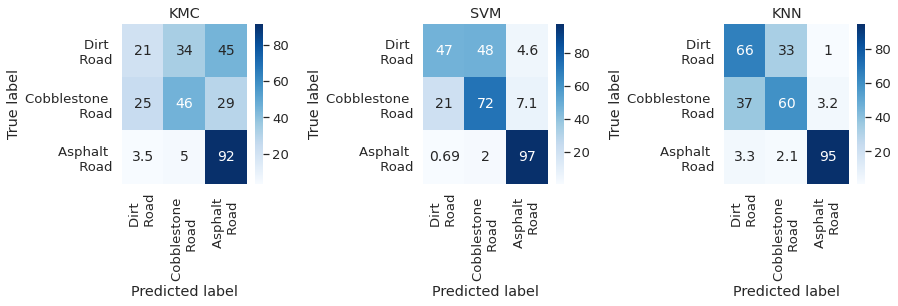
\includegraphics[width=1\textwidth]{figuras/confusion_matrix_classical.png}
  \caption{Matriz de confusão para cada melhor modelo de técnicas clássicas de aprendizado de máquina.}
  \label{fig:confusion_matrix_classical}
\end{figure}

Observando os resultados da Tabela \ref{table:classical_ml_results}, é possível perceber que a técnica de KNN não somente apresenta a maior média de acurácia, como também é a técnica mais estável, com menor variação de resultado entre experimentos com diferentes contextos. O KMC apresenta variância de 18.07\%, o SVM de 14.63\%, e o KNN de 6.85\%. Além disso, observando a matriz confusão dos melhores modelos na Figura \ref{fig:confusion_matrix_classical}, o KNN é a única técnica em que o melhor modelo possuí mais acertos que erros, quando considerado cada tipo de superfície separadamente. Sendo assim, o KNN classificou segmentos de terra com 66\% de acurácia, segmentos de paralelepípedo com 60\% e segmentos de asfalto com 95\%.

Para os experimentos com as técnicas de Deep Learning, inicialmente foram avaliados os diferentes métodos para normalização dos sinais. Dentre os três experimentados, o min-max-scaler entre (0,1) apresentou piores resultados, atingindo maior valor de perda e menor de acurácia. Já o robust-scaler foi o segundo melhor, mantendo sinal nos dados, mas sem escalar em um intervalo. Por fim, os dados normalizados com min-max-scaler entre (-1,1), mantendo o sinal e escalados um intervalo fixo, apresentaram uma convergência mais rápida, menor perda e maior acurácia. Sendo assim, os scalers que mantém o sinal obtiveram resultados melhores, uma vez que o sinal é importante neste estudo, indicando a informação de direção e não apenas uma diminuição de valor. Utilizando os dados normalizados, foram experimentados os modelos de DNN propostos. Os resultados são detalhados nas Tabelas \ref{table:lstm_results}, \ref{table:cnn_results} e \ref{table:cnn_lstm_results}.

\begin{table}[h!]
\caption{Valores de acurácia de validação para DNNs baseados em LSTM.} 
\label{table:lstm_results}
\centering
\small
\begin{tabular}{ccccccc}
\cmidrule(lr){2-6}
 & \multicolumn{5}{c}{\textbf{Janela}} & \multicolumn{1}{c}{} \\ \midrule
\textbf{Model} & \multicolumn{1}{c}{\textbf{100}} & \multicolumn{1}{c}{\textbf{150}} & \multicolumn{1}{c}{\textbf{200}} & \multicolumn{1}{c}{\textbf{250}} & \multicolumn{1}{c}{\textbf{300}} & \multicolumn{1}{c}{\textbf{Média}} \\ \midrule
LSTM 1 & 89.14\% & 89.44\% & \textbf{89.86\%} & 86.30\% & 87.59\% & 88.47\% \\ \midrule
LSTM 2 & \textbf{87.38\%} & 87.33\% & 86.80\% & 86.26\% & 85.85\% & 86.72\% \\ \midrule
LSTM 3 & 89.11\% & 89.61\% & 89.99\% & 89.21\% & \textbf{90.45\%} & 89.67\% \\ \midrule
LSTM 4 & 87.12\% & \textbf{87.31\%} & 87.07\% & 86.11\% & 86.48\% & 86.82\% \\ \midrule
LSTM 5 & 89.74\% & 89.14\% & 90.15\% & \textbf{90.60\%} & 89.63\% & 89.85\% \\ \midrule
LSTM 6 & 88.66\% & 89.69\% & \textbf{90.41\%} & 88.99\% & 90.88\% & 89.72\% \\ \midrule
LSTM 7 & 90.39\% & 91.37\% & 91.85\% & 92.71\% & \textbf{92.73\%} & 91.81\% \\ \midrule
\textbf{Média} & 88.79\% & 89.13\% & 89.45\% & 88.60\% & 89.09\% & 89.01\% \\ \bottomrule
\end{tabular}
\end{table}

\begin{table}[h!]
\caption{Valores de acurácia de validação para DNNs baseados em CNN.} 
\label{table:cnn_results}
\centering
\small
\begin{tabular}{ccccccc}
\toprule
 & \multicolumn{5}{c}{\textbf{Janela}} &  \\ \midrule
\textbf{Model} & \textbf{100} & \textbf{150} & \textbf{200} & \textbf{250} & \textbf{300} & \textbf{Média} \\ \midrule
CNN 1 & 87.44\% & 87.60\% & \textbf{88.25\%} & 87.07\% & 87.54\% & 87.58\% \\ \midrule
CNN 2 & 87.58\% & 87.82\% & 88.25\% & \textbf{88.65\%} & 87.94\% & 88.05\% \\ \midrule
CNN 3 & 89.98\% & 91.67\% & 92.91\% & 92.81\% & \textbf{93.02\%} & 92.08\% \\ \midrule
CNN 4 & 88.88\% & 90.20\% & 91.13\% & 91.78\% & \textbf{92.00\%} & 90.80\% \\ \midrule
CNN 5 & 86.87\% & 87.71\% & \textbf{88.61\%} & 87.81\% & 88.35\% & 87.87\% \\ \midrule
CNN 6 & 90.09\% & 91.12\% & 91.61\% & \textbf{92.17\%} & 91.94\% & 91.39\% \\ \midrule
CNN 7 & 89.17\% & 89.59\% & \textbf{90.14\%} & 89.66\% & 89.65\% & 89.64\% \\ \midrule
CNN 8 & 91.02\% & 91.83\% & 92.89\% & 92.99\% & \textbf{93.17\%} & 92.38\% \\ \midrule
\textbf{Média} & 88.88\% & 89.69\% & 90.47\% & 90.37\% & 90.45\% & 89.97\% \\ \bottomrule
\end{tabular}
\end{table}

\begin{table}[h!]
\caption{Valores de acurácia de validação para DNNs baseados em CNN-LSTM.} 
\label{table:cnn_lstm_results}
\centering
\small
\begin{tabular}{ccccccc}
\toprule
 & \multicolumn{5}{c}{\textbf{Janela}} &  \\ \midrule
\textbf{Model} & \textbf{100} & \textbf{150} & \textbf{200} & \textbf{250} & \textbf{300} & \textbf{Média} \\ \midrule
CNN-LSTM 1 & 87.56\% & 89.15\% & 89.35\% & \textbf{90.97\%} & 90.78\% & 89.56\% \\ \midrule
CNN-LSTM 2 & 87.92\% & 88.38\% & 89.76\% & 89.54\% & \textbf{90.47\%} & 89.21\% \\ \midrule
CNN-LSTM 3 & 87.45\% & 88.77\% & 90.09\% & 89.79\% & \textbf{91.04\%} & 89.43\% \\ \midrule
CNN-LSTM 4 & 87.43\% & 89.43\% & 89.51\% & 89.93\% & \textbf{90.99\%} & 89.46\% \\ \midrule
CNN-LSTM 5 & 90.03\% & 90.69\% & 91.23\% & 91.54\% & \textbf{92.71\%} & 91.24\% \\ \midrule
CNN-LSTM 6 & 90.27\% & 91.50\% & 92.10\% & 92.48\% & \textbf{92.77\%} & 91.82\% \\ \midrule
\textbf{Média} & 88.44\% & 89.65\% & 90.34\% & 90.71\% & 91.46\% & 90.12\% \\ \bottomrule
\end{tabular}
\end{table}

Todos os modelos de DNN propostos, mesmo nos piores resultados, apresentam valor de acurácia de treinamento e validação maior que o melhor modelo baseado em Classical Machine Learning. Isto evidencia a capacidade do Deep Learning aprender relações mais complexas entre os dados, em comparação às técnicas clássicas. Em todos os esperimentos, o impacto na acurácia dado o tamanho da janela de amostras é praticamente insignificante, enquanto que as técnicas clássicas possuem grande variação. Em todas as abordagens de DNN experimentadas, a utilização de Bacth Normalization além de acelerar o treinamento, melhorou os resultados em todos os cenários. A utilização de Dropout também mostrou-se importante para a generalização do modelo. Nos modelos de LSTM-based, a utilização de camadas bidirecionais praticamente não alteraram os resultados, tendo aumento de acurácia para algumas janelas, e diminuição para outras, sempre em valores praticamente irrelevantes e, na média, menores que 1\%. A utilização dos vetores de sequencias da LSTM conectados diretamente nas camadas fully connected pioraram os resultados em todos os experimentos, diminuindo o valor de acurácia em até 4\%. Sendo assim, o modelo LSTM-based com melhores resultados é o LSTM 7, em janela de 300 amostras, onde atingiu valor de acurácia de treinamento de 96.67\% e 92.73\% de acurácia na validação.

Nas redes CNN-based, a utilização de duas a quatro camadas de convolução se mostrou essencial para extração das características. Na saída final dos blocos de convolução para conexão com o bloco de camadas fully connected, a utilização de pooling melhorou os resultados quando comparado a realização apenas de flatten. Tanto max pooling como a global average pool melhoraram resultados, com a segunda sendo significativamente melhor. Sendo assim, todos os experimentos nos quais a média de acurácia das janelas foi maior que 90\%, houve a utilização do global average pool. O modelo de CNN-based com melhores resultados é a CNN 8, com janela de 300 amostras, atingindo acurácia de treinamento de 95.56\% e de 93.17\% na acurácia de validação. Por fim, nas redes CNN-LSTM-based as mesmas considerações da LSTM-based e CNN-based se aplicam, com o melhor modelo sendo a CNN-LSTM 6 com janela de 300 amostras, obtendo acurácia em treinamento de 94.9\% e de 92.77\% de acurácia em validação. Os melhores modelos de DNN para cada abordagem são detalhados na Tabela \ref{table:deep_ml_results}.

\begin{table}[h!]
\caption{Acurácia de validação para cada melhor modelo de técnicas de Deep Learning.} 
\label{table:deep_ml_results}
\centering
\small
\begin{tabular}{cccc}
\toprule
\textbf{Experimento} & 
\textbf{LSTM} & 
\textbf{CNN} & 
\textbf{CNN-LSTM} \\ \midrule
1 & 93.60\% & 94.93\% & 93.68\% \\ \midrule
2 & 91.88\% & 92.25\% & 92.67\% \\ \midrule
3 & 92.70\% & 92.33\% & 91.97\% \\ \midrule
\textbf{Média} & 92.73\% & \textbf{93.17\%} & 92.77\% \\ \bottomrule
\end{tabular}
\end{table}

Com base na Tabela \ref{table:deep_ml_results}, é possível observar as diferentes abordagens de Deep Learning se mostraram adequadas para o problema de classificação de superfície de pista. Avaliando a média de acurácia, o modelo CNN-based foi um pouco melhor que os outros, embora o LSTM-based foi melhor no experimento 3, o CNN-based foi o melhor no experimento 1, e CNN-LSTM-based o melhor no experimento 2, não havendo, portanto, unanimidade. Analisando a matriz confusão da Figura \ref{fig:confusion_matrix_deep}, os segmentos de paralelepípedo são melhor classificados pela LSTM-based, enquanto que o segmentos de asfalto e terra são melhor classificados pela CNN-based e CNN-LSTM-based. Sendo assim, as duas últimas possuem a vantagem de serem mais confiáveis. Analisando estes dois modelos, o valor de acurácia é muito próximo, com a CNN-based sendo relativamente melhor. Contudo, quando avaliado a complexidade do modelo e seu custo computacional, a CNN-LSTM-based tem um custo muito maior. Sendo assim, consideramos a CNN-based o melhor modelo baseado em Deep Learning para classificação de superfície de pista dado sua maior acurácia e menor custo computacional. Desta forma, a técnica classificou segmentos de terra com 93\% de acurácia, segmentos de paralelepípedo com 83\% de acurácia e segmentos de asfalto com 99\% de acurácia, obtendo resultados melhores que os métodos clássicos e que os estudos relacionados, em variação contextual.

\begin{figure}[h!]
  \centering
  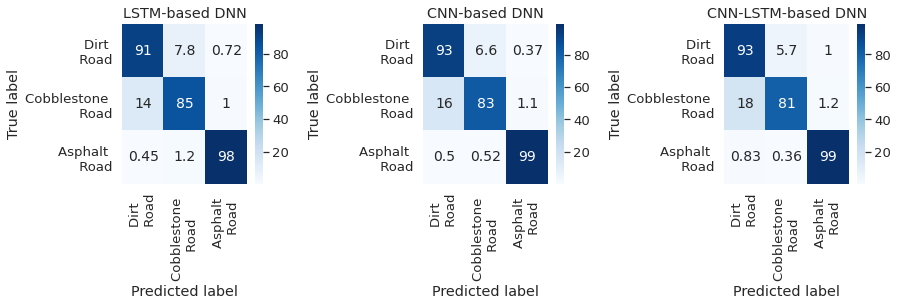
\includegraphics[width=1\textwidth]{figuras/confusion_matrix_deep.png}
  \caption{Matriz de confusão para cada melhor modelo de técnicas de Deep Learning.}
  \label{fig:confusion_matrix_deep}
\end{figure}
